\subsection{Installation}
Get the source code, and make sure VB7, HMMcore, and tools are in your
Matlab path, for example by running the script \verb+vbTPMstart+ from
the Matlab command prompt. (To add these paths permanently to your
Matlab path, see the Matlab documentation).

Make sure that HMMcore/ contains binaries for your system. If not, a
simple Matlab compilation script can be found in HMMcore/. (See Matlab
documentation for how to set up your mex compiler). For large data
sets, it is probably faster to compile your own binaries.

\subsection{System requirements}
Tethered particle motion often produces large data sets of many long
trajectories, which makes the HMM analysis computer intensive. As an
example, one parameter point in our test data sets, about 90
trajectories averaging 45 min, downsampled to 10 Hz, took about 24 h
to go through on two 6 core Intel Xeon E5645 2.40GHz processors. The
analysis time increases sharply with the number of states (including
spurious ones, like transient sticking events).

vbTPM is implemented in Matlab, tested on R2012a and R2013a, and
requires the signal processing and statistics toolbox.

\subsection{A small test problem}
A small test problem can be found in example1/, with the actual data
in example1/lacdata/.  The data set has one calibration (cal) and one
production (trj) trajectory for each bead, and contains data from five
beads. Using the runinput2.m and runscript2.sh files as described
below, this data set takes less than 30 min to analyze on the above
machine (running all five trajectories in parallell).

\subsubsection*{Runinput files} 
Runinput files contain all parameters to run the analysis and access
the results. The meaning of the parameters are documented in the help
text of \verb+VB7_batch_run.m+, and commented in the runinput files in
example1/.  \verb+runinput1.m+ refers to an already completed analysis
(results in example1/HMMresults1/), while \verb+runinput2.m+ has not
yet run.

\subsubsection*{Run basic analysis}
To start analyzing the test data set, type
\verb+VB7_batch_run('runinput2')+ in the Matab command prompt. Since
the runinput file has \verb+one_at_a_time=true;+ this will analyze one
trajectory in the data set. Several calls are needed to complete the
analysis. 

In our experience, Matlab tends to hoard memory if several large data
sets are analyzed consecutively.  To work around that, one can use
scripts that starts consecutive Matlab sessions and runs a single
trajectory in each.

One example for the bash shell is \verb+runscript1.sh+ and
\verb+runscript1.sh+, which calls \verb+runinput1.m+ (there is also a
\verb+runscript2.sh+).

\subsubsection*{Parallelization}
To parallellize, run several instances of the above script at once,
with \verb+one_at_a_time=true;+ in the runinput
file. \verb+VB7_batch_run+ keeps track of which trajectories have
already been 'checked out', so it is also possible to run on several
computers, if the results folder is synced regularly. If the same
trajectory is checked out multiple times on different computers, old
results are simply overwritten (no harm done if they used the same
runinput file).

\subsubsection*{Manage the analysis}
\verb+VB7_batch_manage+ is a tool for managing the basic analysis. It
can collect the results and write them to a file, count how many
trajectories in a data set has been analyzed, and also clean up
temporary files from unfinished trajectories, which is useful if an
analysis run is interrupted.

\subsubsection*{Access the results} 
The GUI for manual state classification is called
\verb+VB7_batch_postprocess()+ (see Fig.~\ref{fig:postprocess}). The
GUI can be used to inspect the analysis results in detail, and can
also convert the simple HMM models to factorial models for further
analysis. To try it out, use the runinput file \verb+runinput1.m+,
which is already analyzed. To access the fitted models directly, use
\verb+VB7_batch_manage+ with the 'collect' option. The results are
returned as cell vectors for calibration and production trajectories,
with the same index structure as the filenames in the runinput file.

For details on how vbTPM represents the models etc., we refer to
section \ref{sec:notation}.

\begin{figure*}
  \begin{center}
    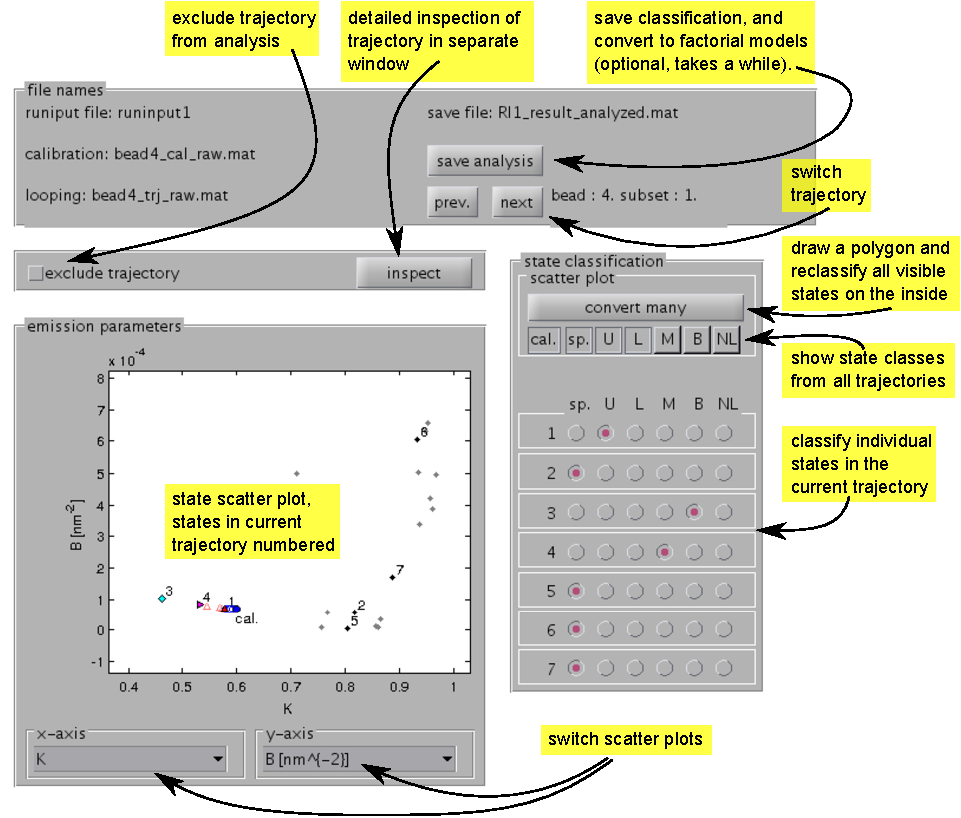
\includegraphics{figures/GUI_manual.pdf}    
  \end{center}
  \caption{Screenshot of the state classification
    GUI.}\label{fig:postprocess}
\end{figure*}
\subsection{Other useful scripts}
\subsubsection{Data and options}
\paragraph{VB7\_getOptions} 
reads a runinput file and return all variables in a struct.
\paragraph{VB7\_preprocess} 
Converts trajectory data to a format that the analysis code
uses. Input trajectory should be drift-corrected.
\paragraph{BWdriftcorrect}
applies driftcorrection to a position trajectory using a Butterworth-filter.
\paragraph{RMSKBgaussfilter}
computes running averages of RMS and other things, using a Gaussian
kernel filter for smoothing.
\paragraph{VB7\_getTrjData} 
returns the data for a single trajectory in a runinput file in various
formats.

\subsubsection{Models}
\paragraph{VB7\_priorParent} 
A tool to initiate models of various sizes with consistent prior
distributions.
\paragraph{VB7\_initialGuess\_KBregion} 
is a rather complicated function to generate an initial guess for a
model struct (e.g., fill out the M and Mc fields) based on analyzing
the data.
\paragraph{VB7\_GSconversion}
is a tool to create factorial models, by converting genuine states
into spurious ones.
\paragraph{VB7\_removeState}
removes states from a model object.
\paragraph{VB7\_findGenuine}
applies a simple set of rules to determine which states in a given
model are genuine and spurious. An analyzed model for the
corresponding calibration trace i also needed to provide a baseline.
\paragraph{VB7\_inspectStates} 
is a simple tool to navigate in the raw data with the help of a
converged model, for example to take a closer look at hard-to-classify
states.

\subsubsection{VB-EM iterations}
\paragraph{VB7\_VBEMiter} 
is the computational core of vbTPM, and runs a single VB-EM iteration.
\paragraph{VB7iterator} 
runs VB-EM iteratons of a model until convergence.
\paragraph{VB7\_greedySearch}
runs a model search on a single trace from a given initial
guess. Briefly, the search strategy is to systematically remove
low-occupancy states until the lower bound $F$ stops increasing.
\paragraph{VB7\_analyzeTrace}
runs several greedy model searches on single traces. 

